\documentclass[main.tex]{subfiles}

\begin{document}
	
	\begingroup
	
	\renewcommand{\cleardoublepage}{}
	
	\renewcommand{\clearpage}{}
	
	\chapter{Grocery Task Overview}
	
	
	\chapterauthor{}
	
	\section{Goal}
	
	\section{Architecture}
	
		\begin{figure}	
			\centering
			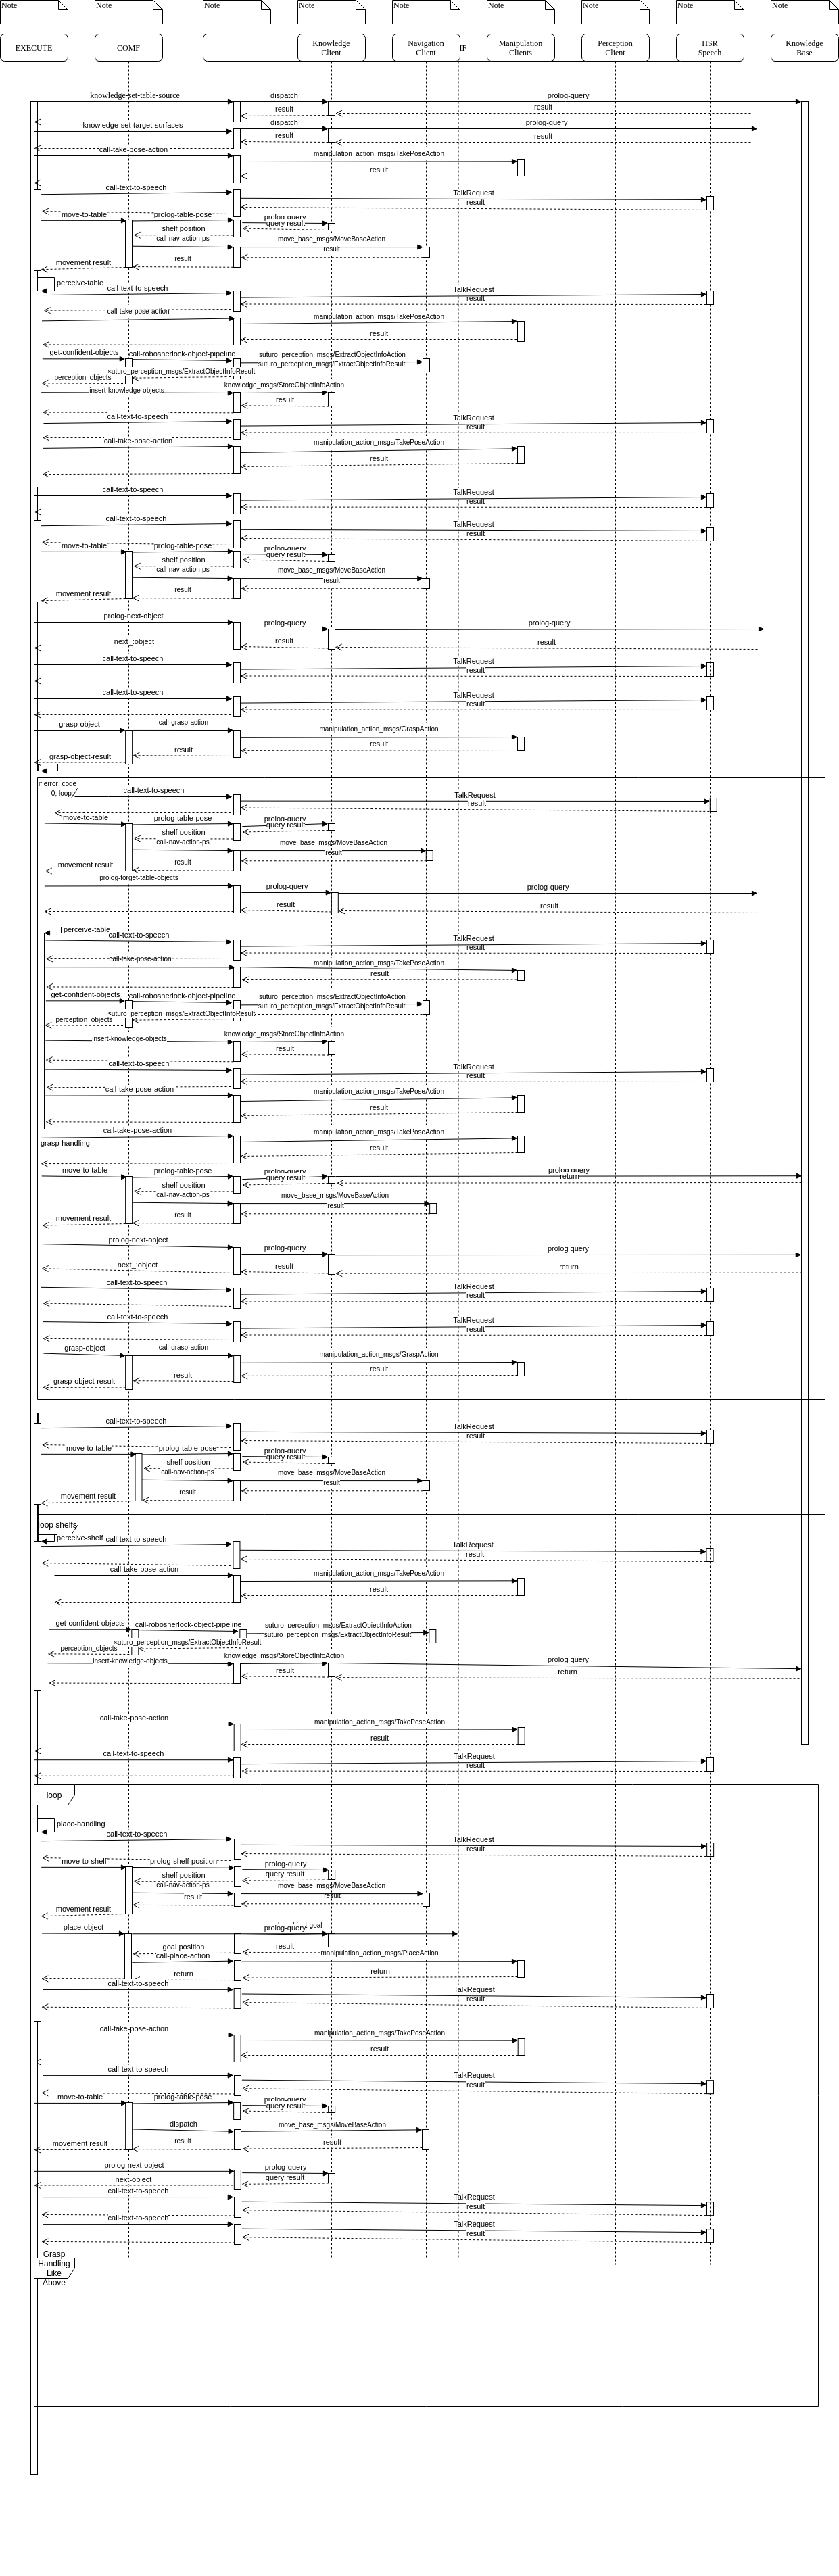
\includegraphics[width=0.7\textwidth]{pictures/diagramms/grocery-sequence.png}
			\caption{}
			\label{fig:grocery-sequence}
		\end{figure}
	
	\section{Description}
	
	\section{sequenzaufgabe}
	hier bitte aus dem sequenz diagramm einen einzelnen task als subsection z.b. schritt: tür öffnen, dafür mussten perception dies tun manipulation das tun etc.
	
	\section{Conclusion}
	
	
	\endgroup
	
\end{document}
